\documentclass{ctexrep}
\usepackage{ctex}
\usepackage{ctexcap}
\usepackage[a4paper,left=2.5cm,right=2cm,top=2.5cm,bottom=2cm]{geometry}
\usepackage{amsmath}
\usepackage{minted}
\usepackage{subfiles}
\usepackage[hidelinks]{hyperref}
\usepackage{xpatch}
\usepackage{graphicx}


\usemintedstyle{vs}

\setminted[cpp]{
frame=lines,
framesep=2mm,
baselinestretch=1.2,
fontsize=\footnotesize,
breaklines,
linenos,
}

\begin{document}
\title{银行管理系统设计报告}
\author{\small 小组独立开发的基于文字界面(TUI)银行管理系统设计报告}
\date{}

\maketitle

% \begin{titlepage}
%   \begin{center}
%     \vfill
%     {\zihao{0} \textbf{银行管理系统设计报告}} \\
%     {\zihao{3}小组独立开发的基于文字界面(TUI)银行管理系统设计报告} \\
%     \vfill
%   \end{center}
% \end{titlepage}

\tableofcontents

\chapter{小组分工}
\input{info.tex}

\chapter{系统分析与设计}
经过小组分析讨论,课程要求中的功能按照操作者可分为三部分。分别是管理部分,
客户业务部分和职员业务部分。

管理部分涉及客户信息的录入和职员信息的录入,较为敏感。而客户业务部分是与客户交互的部分,
这部分应以易用为主,而职员业务部分则为提供给职员进行操作的部分,负责为客户提供相应的服务。
\section{管理部分}
管理部分包含两部分
\begin{itemize}
  \item 银行职员管理:输入数据建立职员表,添加、删除、修改、查询职员信息
  \item 客户账户管理:输入数据建立客户账户表、分账号表,添加、删除、修改、查询客户和账户信息
\end{itemize}

很容易看出这两部分十分相似,都是对数据的 CURD,也就是说经过良好的设计,代码可以进行复用。小组中采用
利用 C++ 的模板,将数据结构抽象为一个链表容器。链表是一个修改为$O(1)$,查找为$O(n)$的线性容器,根据链表的
特性,该容器不支持随机访问(即\mintinline{cpp}{T operator[](std::size_t)}运算符),支持前向迭代器。
其模板定义如下:
\begin{minted}{cpp}
template<typename T>
struct LinkedListNode {
    T data;
    LinkedListNode<T> *next;
    LinkedListNode<T> *prev;
    //...
};
template<typename T>
class LinkedListIter : public std::iterator<std::forward_iterator_tag, T> {
    //...
}
template<typename T>
class LinkedList {
private:
    LinkedListNode<T> *first;
    LinkedListNode<T> *last;
    std::size_t nodeNum;
    //...
}
\end{minted}

银行职员和客户账户的信息很容易明确,其实现时使用结构体进行包装,在开发使用和后续维护中具有
很强的使用价值。系统实现中,为客户信息和职员信息分别建立了 Customer 和 Staff 类用于存放客户信息。

\section{客户业务部分}
\begin{itemize}
  \item 存取贷业务管理:存款、取款、贷款、利息计算、账户余额等
  \item 业务查询:根据不同关键字查询业务信息。
  \item 银行排队管理:分普通客户和VIP客户,排队取号,VIP优先。银行窗口分VIP窗口和普通窗口,一位客户完成业务顺序叫号。客户给职员打分。
  \item 银行网点查询:建立网点地图,查询网点信息,网点导航,网点增删改
\end{itemize}


通过上述的设计,在进行这部分的存取贷业务实现很容易。在进行业务中,只需将业务信息进行储存,
后续便可方便的进行查找。

银行排队管理由于设计普通客户和VIP客户两个窗口,在其中一个队伍为空时会造成资源浪费,因此在设计时的排队如下:


\begin{center}
  \begin{tabular}{|p{3.5cm} p{7.5cm}|}
    当普通队伍和VIP队伍均不为空时 & 普通客户只会前往普通窗口,VIP客户只会前往VIP窗口 \\
    \hline 当普通队伍为空时       & VIP客户可前往VIP窗口或普通窗口                   \\
    \hline 当VIP队伍为空时        & 普通客户可前往普通窗口或VIP窗口
  \end{tabular}
\end{center}

对于网点查询,小组内曾讨论是否能预先使用 SFPA 来求出所有点到终点的最短路,并预先进行存储。但是在后续
的讨论中,考虑到网点会变动,因此移除了 SFPA 而使用 Dijkstra 在运行时求解。

由于地图不应由客户操作,且地图信息较为复杂,因此采用文件的方式存储地图信息。系统在启动时会
读取文件,并根据文件信息初始化地图。

\section{客户资料查询}
\begin{itemize}
  \item 客户资料查询:查询客户资料中的信息,给客户分类
  \item 客户资料管理:建立客户资料文件,存取客户信息
\end{itemize}

很明显这两个都不是由客户进行操作的。客户资料查询可在管理客户资料时对客户信息进行索引,
直接展示客户信息。而客户资料管理则可以直接导出 csv 文件。csv文件作为纯文本的表格,其编辑
处理分类都有其独特的优势。

\chapter{系统创新}
\section{TUI}
该银行管理系统是通过 Win32 控制台运行的,而 Win32控制台是Windows API系统内运行控制台应用程序的文本用户界面的实现。
每个Win32控制台有一个屏幕缓冲区和一个输入缓冲区,并可在窗口下使用。输入缓冲区是一个存储事件的队列,事件来自键盘、鼠标等。
输出缓冲区是一个存储字符以及其属性的网格矩阵。一个控制台窗口可能有多个输出缓冲区,但同一时刻只有一个能处于活动状态(即显示)。
根据上述特点,稍化功夫就可以实现一个TUI框架。

小组通过对缓冲区的直接操作,实现了一个TUI框架。
\begin{figure}[!h]
  \centering
  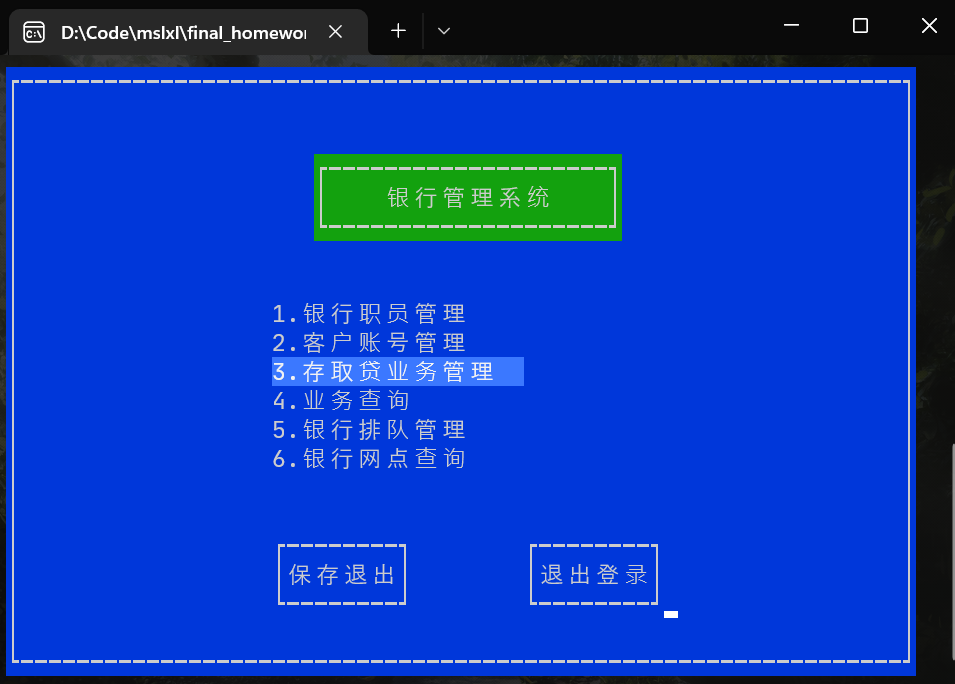
\includegraphics[scale=0.45]{main_meun.png}
  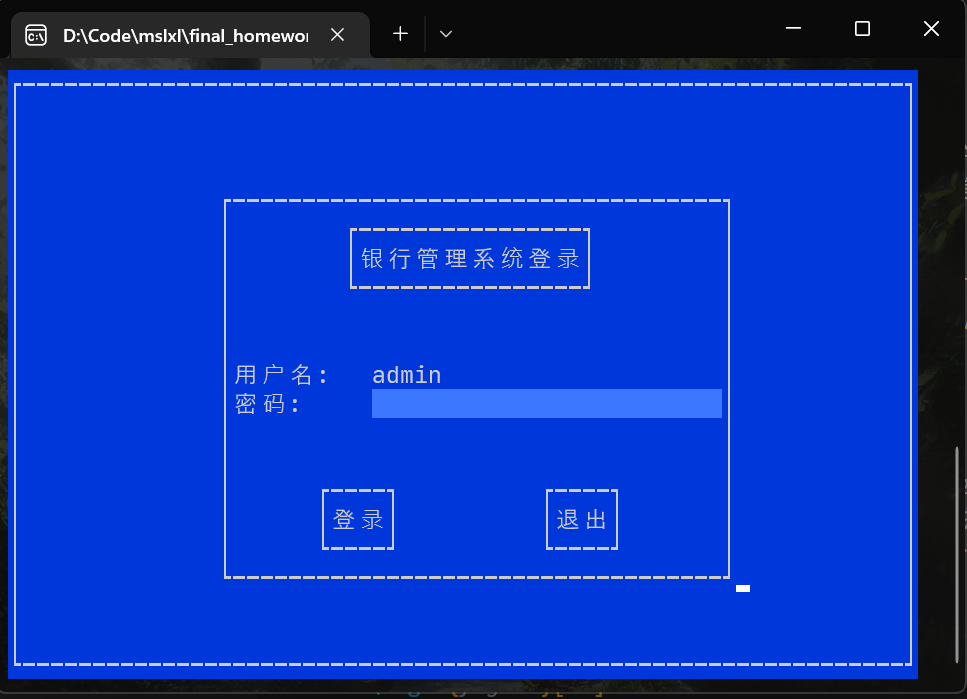
\includegraphics[scale=0.45]{login.png}
  \caption{TUI展示}
\end{figure}

不同与传统的 UI 框架,该框架采用声明式布局,数据更新方式参考了 MVVM 架构,通过监听器(自动构建)
同步数据与界面。界面的布局代码实际会构建一棵树(如图3.2),程序将对其进行 DFS 以测量组件大小,并在测量结束后
在控制台缓冲区进行绘制。
\begin{figure}[!h]
  \centering
  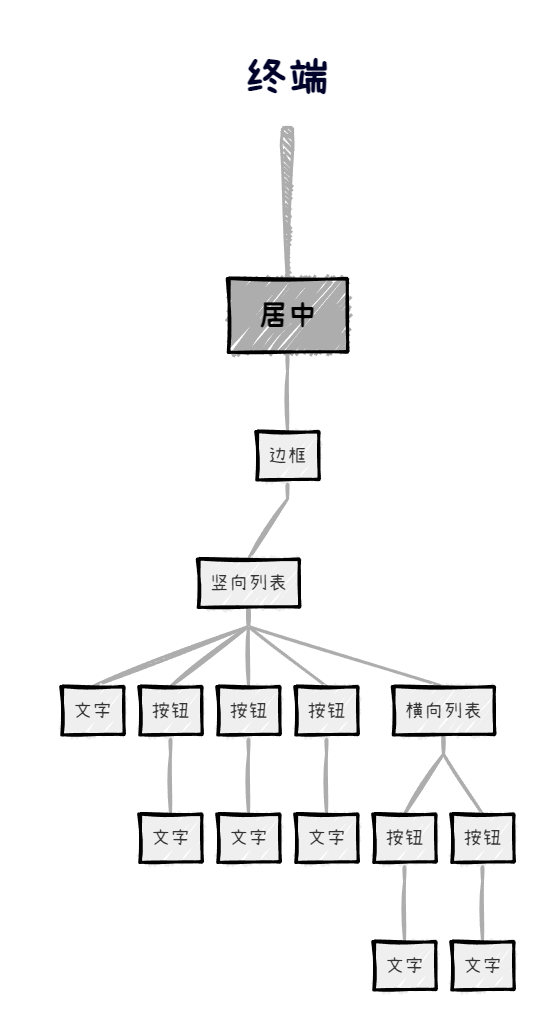
\includegraphics[scale=0.5]{tree.png}
  \caption{组件树}
\end{figure}
组件拥有三种大小:
\begin{itemize}
  \item 固定大小(如 Text)
  \item 自适应大小(如 ListView)
  \item 全屏(如 Center)
\end{itemize}

组件为自适应大小时,组件会主动测量其自节点的大小,并通过计算求出能满足子节点的最小大小,
以此作为自身大小。全屏的组件则不理会子节点的大小,而是尽可能的大,占据其父节点的所有大小。

这里其实存在一个问题,如果一个组件大小为自适应,其子节点大小为全屏,此时会出现死循环。
因此,小组提出了“二次测量”方案,通过$O(2^n)$这个比较大的消耗解决了问题,在组件数目不多的
情况下,这个时间复杂度是完全可以接受的。

在二次测量中,父组件将先用 $(0,0)$ 对所有子组件进行测量,在测量结束后计算其最小大小,再用最小大小 $(a,b)$ 去
二次测量所有组建,通过这种方式,该TUI框架实现了极其方便的布局。

\section{Wildcard模糊查找}
生活中,显然有些东西并不是十分清楚的,在信息管理中也一样。有时我们需要对某些信息进行
模糊查找匹配,因此小组实现了 Wildcard模糊匹配


其实现逻辑十分简单。通过逐位对比,当匹配时进行匹配下一位。当遇到 $*$ 或 $?$, $.$ 等通配符时,
优先尝试尽可能多的匹配(即贪婪匹配),若后续匹配中发生失败,则进入 panic 状态处理错误,试图用
回溯恢复错误状态。\input{name1.txt}表示这些思路来自于编译原理课程中的 $LL(k)$ CFG 文法,经实战表示该思路可行。

\begin{minted}[highlightlines={20-52}]{cpp}
//
// Created by mslxl on 11/23/2022.
//

#include <cctype>
#include <iterator>
#include <string>
  namespace details {
        template<typename Compare,
                typename Iterator,
                typename ValueType = typename std::iterator_traits<Iterator>::value_type>
        inline bool match_impl(const Iterator pattern_begin,
                               const Iterator pattern_end,
                               const Iterator data_begin,
                               const Iterator data_end,
                               const ValueType zero_or_more,
                               const ValueType exactly_one) {
            typedef typename std::iterator_traits<Iterator>::value_type type;

            const Iterator null_itr(0);

            Iterator p_itr = pattern_begin;
            Iterator d_itr = data_begin;
            Iterator np_itr = null_itr;
            Iterator nd_itr = null_itr;

            for (;;) {
                if (pattern_end != p_itr) {
                    const type c = *(p_itr);

                    if ((data_end != d_itr) && (Compare::cmp(c, *(d_itr)) || (exactly_one == c))) {
                        ++d_itr;
                        ++p_itr;
                        continue;
                    } else if (zero_or_more == c) {
                        while ((pattern_end != p_itr) && (zero_or_more == *(p_itr))) {
                            ++p_itr;
                        }

                        const type d = *(p_itr);

                        while ((data_end != d_itr) && !(Compare::cmp(d, *(d_itr)) || (exactly_one == d))) {
                            ++d_itr;
                        }

                        // set backtrack iterators
                        np_itr = p_itr - 1;
                        nd_itr = d_itr + 1;

                        continue;
                    }
                } else if (data_end == d_itr)
                    return true;

                if ((data_end == d_itr) || (null_itr == nd_itr))
                    return false;

                p_itr = np_itr;
                d_itr = nd_itr;
            }
        }

        typedef char char_t;

        struct cs_match {
            static inline bool cmp(const char_t c0, const char_t c1) {
                return (c0 == c1);
            }
        };

        struct cis_match {
            static inline bool cmp(const char_t c0, const char_t c1) {
                return (std::tolower(c0) == std::tolower(c1));
            }
        };

    }

    inline bool match(const std::string &str,
                      const std::string &pattern,
                      const std::string::value_type match_one_or_more = '*',
                      const std::string::value_type match_exactly_one = '.') {
        return details::match_impl<details::cs_match>
                (
                        std::cbegin(pattern), std::cend(pattern),
                        std::cbegin(str), std::cend(str),
                        match_one_or_more,
                        match_exactly_one
                );
    }
\end{minted}

\section{AES}
\chapter{功能实现}

\begin{enumerate}
\item 进入系统后会首先进行银行管理系统的初始化。初始化进入系统之后会显示功能列表,可选择任意子系统。
\item 进入银行职员管理系统后可以浏览职员信息,如没有数据可以进行职员数据的添加、查找、更改、删除。
\item 进入客户账户管理子系统后,首先浏览客户信息,如没有数据可以进行职员数据的添加、查找、更改、删除。
\item 选择进入存取贷款业务管理子系统应该输入正确的卡号与密码进入,之后可以进行存款、取款、贷款、还款的业务,在办理贷款业务后,也会进行一定的利息计算,同时可可以进行账户余额的查询。
\item 进入客户资料管理的子系统后首先进行客户资料的统揽,若无信息则可选择添加客户资料,添加客户资料包括客户的账号、户名、密码、邮箱、电话以及是否为VIP客户。
\item 进入银行网点管理子系统首先进行银行网点信息的浏览,也可以进行网点信息的添加,包括网点编号、公司名称、电话、地址。返回上一界面后可以选择搜索网点,可以通过网点编号、公司名称、电话、地址以及可以进行一些模糊搜索。搜索完成后可以通过输入网点编号对网点信息进行修改与删除。
\item 通过业务查询子系统可以通过输入关键字对各个子系统功能进行搜索。
\item 进入银行排队系统管理系统后,客户应选择客户排队通过输入账户进行排队,同时系统会判断是否为VIP客户,如果是则优先排队,反之正常。在业务办理完成后客户还会进行打分评价。
\end{enumerate}
\chapter{总结与体会}
\input{suffix.tex}

\end{document}
